%\documentclass[twoside,a4paper]{report}
\documentclass[a4paper]{article}

\usepackage[utf8]{inputenc}

\usepackage{hyperref}
\usepackage{graphicx}
\usepackage{tabularx}
\usepackage{supertabular}
\usepackage{pdflscape} %% Used for very big table
\usepackage{moreverb}
\usepackage[table]{xcolor}
\usepackage{listings}
\usepackage{fancyhdr}
\usepackage[draft]{fixme}

\definecolor{codegray}{gray}{.95}
\definecolor{palegray}{gray}{.65}
\lstset{language=C,
	numbers=left,
	tabsize=2,
	basicstyle=\scriptsize,
	stringstyle=\textrm,
	showstringspaces=false,
	frame=none,
	xleftmargin=3pt,
	backgroundcolor=\color{codegray}}

\title{Current State of Knowledge Representation Systems for Robotics}
\author{Séverin Lemaignan, Moritz Tenorth}

\graphicspath{{figs/}}

\begin{document}

\maketitle
\tableofcontents

\section{Introduction}
\label{sect|intro}

\subsection{Definition of inclusion criteria}

We have setup the following criteria to select the knowledge representation
systems to include in this survey.

Those systems must:

\begin{itemize}
	\item  Run on \emph{service robot} (robots that interact with objects in a
	semantic-rich environment),

	\item  Ground their knowledge in the physical world (physically embedded),
	\begin{itemize}
		\item  Able to \emph{resolve entities}
		\item  Able to automatically create new object instances
	\end{itemize}

	\item  Be able to merge different knowledge modalities,
	\item  Be endowed with on-line, dynamic reasoning (not just a static
	dictionary)

\end{itemize}

\subsection{Methodology}
\label{sect|methodology}


\fxnote{Mention here that each team was proposed to complete/amend the description of their
system}
	
\section{Comparison criteria}
\label{sect|comparison-criteria}

\subsection{Intrinsic features}
\label{sect|intrinsic-features}

\begin{itemize}
	\item  Expressiveness
	\begin{itemize}
		\item  Which logic formalism (DL, 2nd order\ldots{})
		\item  OWA/CWA
		\item  Representation of uncertainty
		\item  (non) monotonic reasoning
		\item  General knowledge + exception to this knowledge (blue sky/white sky)
		\item  Microtheories
		\item  Lazy evaluation
		\item  Presupposition accomodation (ability to represent facts that are only verbally hinted, but not grounded into perception)
	\end{itemize}

	\item  Explicit modeling of context of knowledge / domain of validity
	\item  Representation of change (\emph{"The pancake dough disappears into a pancake"})
	\item  Support for learning
	\item  Support for introspection?
	\item  Support for prediction/projection?
\end{itemize}

\subsection{Strategies to deal with the physical world}

\begin{itemize}
	\item  Knowledge acquisition possible\ldots{}
	\begin{itemize}
		\item  \ldots{}through interaction? How?
		\item  \ldots{}through the Web? How?
		\item  \ldots{}through learning? How?
		\item  \ldots{}through perception? How?
	\end{itemize}
	\item Grounding/anchoring strategies
	\item Ability to automatically create new object instances
	\item Ability to merge modalities
\end{itemize}

\subsection{Integration in a larger robotic architecture}

\begin{itemize}

	\item  Integration with executive layers
	\begin{itemize}
		\item  Events
		\item  Relation to task planning
	\end{itemize}

	\item  Scalability and responsiveness
\end{itemize}

\subsection{Underlying knowledge model}

\begin{itemize}
	\item  Which underlying knowledge (\emph{common-sense}, \emph{upper knowledge}\ldots{})
	\begin{itemize}
		\item  top-down approach?
	\end{itemize}

\end{itemize}

\section{Surveyed systems}

Table \ref{table|surveyed-systems} presents the fifteen knowledge representation systems surveyed
in this article.

This section briefly presents each of them.

\begin{landscape}
\begin{table}
\begin{center}
\rowcolors{2}{lightgray}{codegray}

%\begin{tabularx}{\textheight}{p{2cm}p{4cm}p{3cm}p{4cm}p{2.3cm}p{2cm}p{2cm}}
\begin{tabular}{lllllll}
\hiderowcolors
{\bf Project} & {\bf Authors (Institution)} & {\bf Project homepage} & {\bf Programming language} & {\bf Knowledge model} & {\bf Reasoner} & Main reference \\
\hline
\showrowcolors
{\sc KnowRob} & Tenorth (TU Munich) & & {\sc Prolog} & {\sc Prolog} + OWL-DL & Custom ({\sc Prolog}) & \cite{Tenorth2009a} \\
ORO & Lemaignan (LAAS-CNRS) & \url{oro.openrobots.org} & {\sc Java} & OWL-DL ({\sc Jena}) & {\sc Pellet} & \cite{Lemaignan2010} \\
PEIS Ecology & Daoutis, Coradeshi, Loutfi, Saffiotti (Örebro Univ.) & \url{www.aass.oru.se/~peis} & {\sc C}, {\sc CycL} & OWL-Full, 2nd order logics & & \cite{Daoutis2009} \\
 & Kollar, Tellex \\
OMKRF \\
 & Roy, Mavridis \\
 & Wrighteagle \\
 & Vincze \\
 & (Bielfeld) \\
ARMAR & Schmidt-Rohr (Karlsruhe) \\
 & (Saarbrücken) \\
 & Hertzberg (Osnabrück) \\
 & (DFKI Bremen) \\
 (based on {\sc KnowRob} & (JSK) \\
DY-KNOW & Heitnz, Dowerty \\

\hline

%\end{tabularx}
\end{tabular}
\end{center}
\caption{List of surveyed systems}
\label{table|surveyed-systems}
\end{table}
\end{landscape}

\subsection{PEIS Ecology}
\label{sect|peis-ecology}

Reference paper:~\cite{Daoutis2009}

{\sc PEIS Ecology}~\cite{Saffiotti2005} is a software \emph{ecosystem} that aim to binds autonomous
robotics with ambient intelligence (network of sensors). \emph{PEIS} stands for
\emph{Physically Embedded Intelligent System}: every robots or intelligent
device in the environment is abstracted as a PEIS.

Each PEIS component is running a \emph{PEIS Kernel} instance. Communication
between instance relies on a custom P2P communication protocol.

In short:
* Roughly the same kind of ambition and architecture.
* Way better than us on the perception side. 
* They try the "2nd order logic" approach. I'd be curious to know what kind of reasoning capability they actually have.
* Their tests are conducted in a static environment. They don't take other agents into consideration (nothing like perspective taking or rich disambiguation).
* No task planning at all (or at least, not discussed in this paper)

More in details:
- object identification based on viewpoint independent SIFT features
- formalized anchoring system that explicitely match percieved attributes to predicates
- Cyc predicates
- ground 12 colors, based on a paper on color perception. Could be useful for us.
- idem, they cite a paper on what spatial relations to compute
- location of objects based on a previously provided semantic map (but not much on this semantic map)
- two "memories": the robot memory stores the current list of percieved objects ; the archive memory stores what is not percieved anymore
- uses directly Cyc (ie, 250 000 common sense concepts...), via CycL language -> 2nd and higher order logics (quantification over predicates, functions, etc)
Remark: using 2nd order logic (ie meta statements), it would be easy to store the knowledge of each agent
- disambiguation in concept name by asking human to decide amongst all concepts known by Cyc
- template based natural language
- experiment conducted in a "smart" indoor environmement + simple robot

\subsubsection{Intrinsic features}
\label{sect|peis-intrinsic-features}

\subsubsection{Integration in the PEIS Ecology architecture}
\label{sect|peis-integration}

\begin{figure}
	\centering
	\includegraphics[width=0.9\columnwidth]{peis-architecture.pdf}
	\caption{The PEIS knowledge representation system, taken from~\cite{Daoutis2009}}
	\label{fig|peis-architecture}
\end{figure}

The PEIS KR\&R system is deeply integrated to the general PEIS Ecology environment.



\begin{table}
\begin{center}
\rowcolors{2}{lightgray}{codegray}

\begin{tabular}{ll}
\hiderowcolors
{\bf Project} & {\bf Common-sense knowledge source} \\
\hline
\showrowcolors
{\sc KnowRob} & {\sc OpenCyc}, processed web content, custom OWL-DL ontology \\
ORO & {\sc OpenCyc}, custom OWL-DL ontology \\
PEIS Ecology & {\sc ReseachCyc} \\
 & Kollar, Tellex \\
OMKRF \\
 & Roy, Mavridis \\
 & Wrighteagle \\
 & Vincze \\
 & (Bielfeld) \\
ARMAR & Schmidt-Rohr (Karlsruhe) \\
 & (Saarbrücken) \\
 & Hertzberg (Osnabrück) \\
 & (DFKI Bremen) \\
 (based on {\sc KnowRob} & (JSK) \\
DY-KNOW & Heitnz, Dowerty \\

\hline

\end{tabular}
\end{center}
\caption{Underlying knowledge sources for each project}
\label{table|knowledge-sources}
\end{table}


\section{Conclusion}
\label{sect|conclusion}

\subsection{Main groups}

\subsection{What is not successfully covered by current systems}

\subsection{Future challenges}
\label{sect|future-challenges}

%%%%%%%%%%%%%%%%%%%%%%%%%%%%%%%%%%%%%%%%%%%%%%%%%%%%%%%%%%%%%%%%%%%%%%%%%% 
\section*{Acknowledgements} 

%%%%%%%%%%%%%%%%%%%%%%%%%%%%%%%%%%%%%%%%%%%%%%%%%%%%%%%%%%%%%%%%%%%%%%%%%% 

\bibliographystyle{ieeetr}
\bibliography{biblio}


\end{document}
